\documentclass[11pt]{article}

\usepackage[margin=1in]{geometry}
\usepackage{amsmath, amssymb}
\usepackage{graphicx}
\usepackage{booktabs}
\usepackage{longtable}
\usepackage{hyperref}

\title{Pet Cafe Management System\\Design Document}
\author{Nathan Tebbs \and Krish Patel \and CJ De Vault \and Shayden Lowry}
\date{December 8, 2025}

\begin{document}
\maketitle

\tableofcontents
\newpage

% ==========================================================
% 1. CONCEPTUAL DATABASE DESIGN
% ==========================================================
\section{Conceptual Database Design}

\subsection{Overview of the Data Model}

The Pet Cafe Management System manages members, pets, staff, rooms, reservations, visits,
food \& beverage orders, events, and adoptions. The goal is to support safe interactions
between customers and animals, track cafe revenue, and manage operational constraints
such as room capacity and pet health requirements.

At a high level, the main entity groups are:
\begin{itemize}
    \item Customer--facing entities: \textbf{Member}, \textbf{Reservation}, \textbf{Visit}, \textbf{Order}, \textbf{Event}, \textbf{EventRegistration}.
    \item Pet--related entities: \textbf{Pet}, \textbf{HealthRecord}, \textbf{BehavioralAssessment}, \textbf{AdoptionApplication}, \textbf{AdoptionRecord}.
    \item Cafe operations: \textbf{MenuItem}, \textbf{OrderItem}, \textbf{Room}, \textbf{Staff}.
    \item Membership management: \textbf{MembershipTier}, \textbf{MembershipPayment}.
\end{itemize}

\subsection{E--R Diagram}

Figure~\ref{fig:er} shows the final E--R diagram for the system.

\begin{figure}[h]
    \centering
    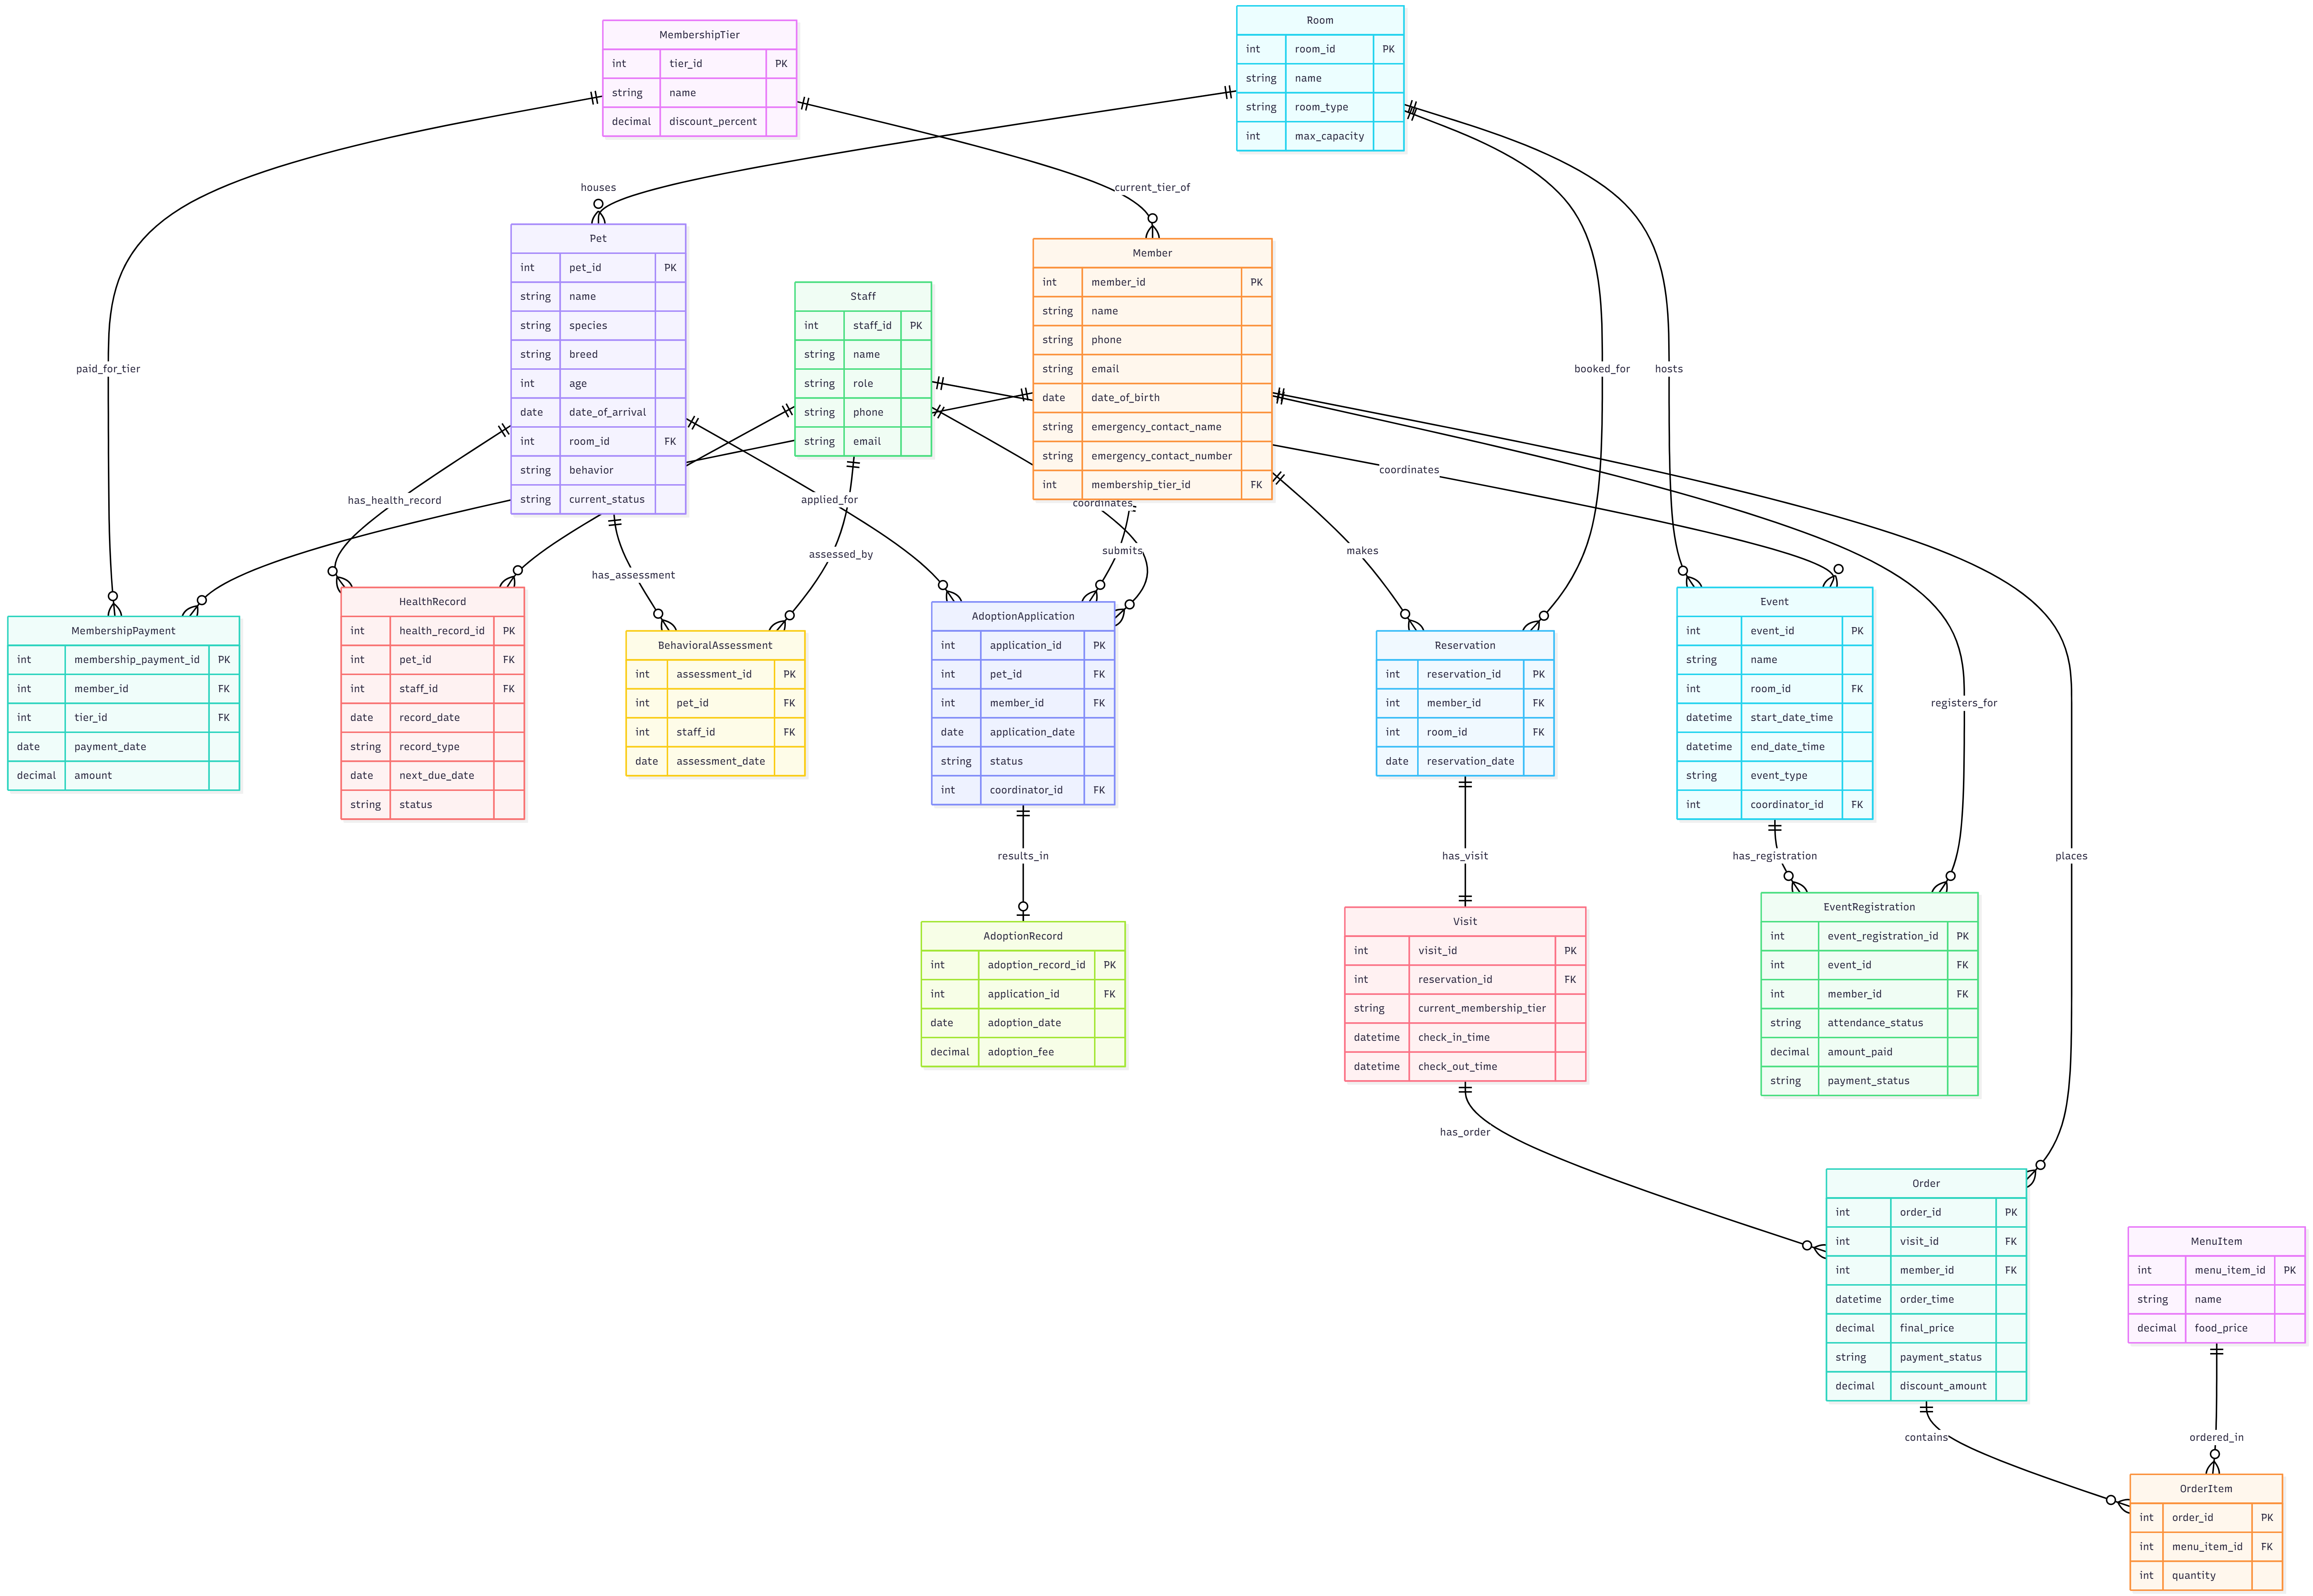
\includegraphics[width=\textwidth]{Final ER Diagram.png}
    \caption{Final E--R Diagram for the Pet Cafe Management System}
    \label{fig:er}
\end{figure}

\subsection{Entity Descriptions}

Below is a brief description of the key entities and their roles in the system.

\paragraph{Member}
Represents a registered customer. Each Member has contact information, a date of birth,
and an assigned membership tier. Members can create reservations, attend events,
submit adoption applications, and generate visits and orders indirectly.

\paragraph{MembershipTier}
Defines membership levels such as Day Pass, Monthly, and Annual.
The tier determines the discount percentage applied to eligible cafe orders and events.

\paragraph{MembershipPayment}
Records payments made by members for their membership tiers. Each payment is associated
with one Member and one MembershipTier.

\paragraph{Staff}
Represents employees and volunteers, including veterinary staff, pet handlers,
baristas, adoption coordinators, and event coordinators.

\paragraph{Room}
Represents a physical space in the cafe, such as a cat lounge or event room.
Reservations and events are associated with rooms, and pets can be housed in rooms.

\paragraph{Pet}
Represents an animal living at or managed by the cafe. Pets have health and behavioral
information, can be available for adoption, and may have adoption applications and
adoption records.

\paragraph{HealthRecord}
Stores medical and care information for pets (vaccinations, checkups, grooming, etc.).
Each record is tied to a Pet and the Staff member who recorded it.

\paragraph{BehavioralAssessment}
Stores behavioral evaluations for pets, performed by Staff members.

\paragraph{AdoptionApplication}
Represents a request by a Member to adopt a specific Pet, coordinated by a Staff member.
Applications move through statuses such as pending, approved, rejected, or withdrawn.

\paragraph{AdoptionRecord}
Represents a finalized adoption tied to a single AdoptionApplication.

\paragraph{Reservation}
Represents a booking made by a Member for a specific Room and time slot.
Each Reservation may result in exactly one Visit.

\paragraph{Visit}
Represents an actual check--in/check--out window for a Reservation.
Visits are the anchor for Orders and store a snapshot of the member's membership tier.

\paragraph{MenuItem}
Represents a food or beverage item on the cafe menu, including price and category.

\paragraph{Order}
Represents a food \& beverage order placed during a Visit.
An Order has one or more OrderItems.

\paragraph{OrderItem}
Represents a line item in an Order: which MenuItem, quantity, and price charged.

\paragraph{Event}
Represents an event such as a workshop or adoption event, hosted in a Room
and coordinated by a Staff member.

\paragraph{EventRegistration}
Represents a Member's registration for an Event, including attendance and payment status.

\subsection{Key Design Rationale and Constraints}

\subsubsection{Normalization and Order--Member Relationship}

In the conceptual domain, an order is clearly associated with the customer who
placed it. However, in the normalized schema we do \emph{not} store \texttt{member\_id}
directly in \textbf{Order}. Instead, we derive it via:
\[
    \text{Order} \rightarrow \text{Visit} \rightarrow \text{Reservation} \rightarrow \text{Member}.
\]
Storing \texttt{member\_id} in Order would introduce functional dependency redundancy
and violate BCNF; removing it keeps the schema clean while still answering all
business queries.

\subsubsection{Visit and Membership Tier Snapshot}

We store \texttt{current\_membership\_tier} in \textbf{Visit} as a snapshot.
This preserves the membership tier used for pricing at the time of the visit,
even if the member upgrades or downgrades later.

\subsubsection{Legal and Historical Records}

Medical records and adoption history are legally and operationally important.
\textbf{HealthRecord} rows are never physically deleted; instead, entries made in error
are marked as void or corrected at the application level. Similarly, adoption
applications and records are retained even if an application is withdrawn.

\subsubsection{Capacity and Safety Constraints}

Room capacity, event capacity, and pet availability constraints are modeled
at the conceptual level and enforced in application logic (and where possible,
through database constraints and checks).

\newpage

% ==========================================================
% 2. LOGICAL DATABASE DESIGN
% ==========================================================
\section{Logical Database Design}

This section describes the relational schemas derived from the conceptual design.

\subsection{Relational Schemas}

Below we list each relation in the final logical schema. Attribute names and
types correspond to the implementation in Oracle.

\subsubsection*{Member}
\begin{verbatim}
Member(
    member_id           NUMBER        PK,
    name                VARCHAR2(100) NOT NULL,
    phone               VARCHAR2(20)  NOT NULL,
    email               VARCHAR2(100) NOT NULL,
    date_of_birth       DATE          NOT NULL,
    emergency_contact_name   VARCHAR2(100),
    emergency_contact_number VARCHAR2(20),
    membership_tier_id  NUMBER        NOT NULL  FK -> MembershipTier(tier_id)
)
\end{verbatim}

\subsubsection*{MembershipTier}
\begin{verbatim}
MembershipTier(
    tier_id          NUMBER        PK,
    name             VARCHAR2(50)  NOT NULL UNIQUE,
    discount_percent NUMBER(5,2)   NOT NULL
)
\end{verbatim}

\subsubsection*{MembershipPayment}
\begin{verbatim}
MembershipPayment(
    membership_payment_id NUMBER      PK,
    member_id             NUMBER      NOT NULL FK -> Member(member_id),
    tier_id               NUMBER      NOT NULL FK -> MembershipTier(tier_id),
    payment_date          DATE        NOT NULL,
    amount                NUMBER(8,2) NOT NULL
)
\end{verbatim}

\subsubsection*{Staff}
\begin{verbatim}
Staff(
    staff_id    NUMBER        PK,
    name        VARCHAR2(100) NOT NULL,
    role        VARCHAR2(50)  NOT NULL,
    phone       VARCHAR2(20)  NOT NULL,
    email       VARCHAR2(100) NOT NULL
)
\end{verbatim}

\subsubsection*{Room}
\begin{verbatim}
Room(
    room_id      NUMBER        PK,
    name         VARCHAR2(50)  NOT NULL,
    room_type    VARCHAR2(30)  NOT NULL,
    max_capacity NUMBER        NOT NULL
)
\end{verbatim}

\subsubsection*{Pet}
\begin{verbatim}
Pet(
    pet_id         NUMBER        PK,
    name           VARCHAR2(50)  NOT NULL,
    species        VARCHAR2(30)  NOT NULL,
    breed          VARCHAR2(50),
    age            NUMBER,
    date_of_arrival DATE         NOT NULL,
    room_id        NUMBER        FK -> Room(room_id),
    temperament    VARCHAR2(100),
    special_needs  VARCHAR2(200),
    current_status VARCHAR2(30)  NOT NULL
)
\end{verbatim}

\subsubsection*{HealthRecord}
\begin{verbatim}
HealthRecord(
    health_record_id NUMBER       PK,
    pet_id           NUMBER       NOT NULL FK -> Pet(pet_id),
    staff_id         NUMBER       NOT NULL FK -> Staff(staff_id),
    record_date      DATE         NOT NULL,
    record_type      VARCHAR2(50) NOT NULL,
    next_due_date    DATE,
    status           VARCHAR2(30) NOT NULL
)
\end{verbatim}

\subsubsection*{BehavioralAssessment}
\begin{verbatim}
BehavioralAssessment(
    assessment_id   NUMBER        PK,
    pet_id          NUMBER        NOT NULL FK -> Pet(pet_id),
    staff_id        NUMBER        NOT NULL FK -> Staff(staff_id),
    assessment_date DATE          NOT NULL,
    notes           VARCHAR2(4000)
)
\end{verbatim}

\subsubsection*{AdoptionApplication}
\begin{verbatim}
AdoptionApplication(
    application_id   NUMBER        PK,
    pet_id           NUMBER        NOT NULL FK -> Pet(pet_id),
    member_id        NUMBER        NOT NULL FK -> Member(member_id),
    coordinator_id   NUMBER        NOT NULL FK -> Staff(staff_id),
    application_date DATE          NOT NULL,
    status           VARCHAR2(30)  NOT NULL
)
\end{verbatim}

\subsubsection*{AdoptionRecord}
\begin{verbatim}
AdoptionRecord(
    adoption_record_id NUMBER      PK,
    application_id     NUMBER      NOT NULL FK -> AdoptionApplication(application_id),
    adoption_date      DATE        NOT NULL,
    adoption_fee       NUMBER(8,2) NOT NULL
)
\end{verbatim}

\subsubsection*{Reservation}
\begin{verbatim}
Reservation(
    reservation_id   NUMBER       PK,
    member_id        NUMBER       NOT NULL FK -> Member(member_id),
    room_id          NUMBER       NOT NULL FK -> Room(room_id),
    reservation_date DATE         NOT NULL,
    start_time       TIMESTAMP    NOT NULL,
    end_time         TIMESTAMP    NOT NULL,
    status           VARCHAR2(20) NOT NULL
)
\end{verbatim}

\subsubsection*{Visit}
\begin{verbatim}
Visit(
    visit_id                NUMBER        PK,
    reservation_id          NUMBER        NOT NULL FK -> Reservation(reservation_id),
    current_membership_tier VARCHAR2(50)  NOT NULL,
    check_in_time           TIMESTAMP     NOT NULL,
    check_out_time          TIMESTAMP
)
\end{verbatim}

\subsubsection*{MenuItem}
\begin{verbatim}
MenuItem(
    menu_item_id NUMBER        PK,
    name         VARCHAR2(100) NOT NULL UNIQUE,
    food_price   NUMBER(6,2)   NOT NULL,
    category     VARCHAR2(50)  NOT NULL,
    description  VARCHAR2(200)
)
\end{verbatim}

\subsubsection*{Order}
\begin{verbatim}
Order(
    order_id        NUMBER        PK,
    visit_id        NUMBER        NOT NULL FK -> Visit(visit_id),
    order_time      TIMESTAMP     NOT NULL,
    final_price     NUMBER(8,2)   NOT NULL,
    payment_status  VARCHAR2(20)  NOT NULL,
    discount_amount NUMBER(8,2)   NOT NULL
)
\end{verbatim}

\subsubsection*{OrderItem}
\begin{verbatim}
OrderItem(
    order_id     NUMBER      NOT NULL FK -> Order(order_id),
    menu_item_id NUMBER      NOT NULL FK -> MenuItem(menu_item_id),
    quantity     NUMBER      NOT NULL,
    item_price   NUMBER(6,2) NOT NULL,
    PRIMARY KEY (order_id, menu_item_id)
)
\end{verbatim}

\subsubsection*{Event}
\begin{verbatim}
Event(
    event_id        NUMBER        PK,
    name            VARCHAR2(100) NOT NULL,
    event_type      VARCHAR2(50)  NOT NULL,
    room_id         NUMBER        NOT NULL FK -> Room(room_id),
    start_date_time TIMESTAMP     NOT NULL,
    end_date_time   TIMESTAMP     NOT NULL,
    coordinator_id  NUMBER        NOT NULL FK -> Staff(staff_id)
)
\end{verbatim}

\subsubsection*{EventRegistration}
\begin{verbatim}
EventRegistration(
    event_registration_id NUMBER       PK,
    event_id              NUMBER       NOT NULL FK -> Event(event_id),
    member_id             NUMBER       NOT NULL FK -> Member(member_id),
    attendance_status     VARCHAR2(20) NOT NULL,
    amount_paid           NUMBER(8,2)  NOT NULL,
    payment_status        VARCHAR2(20) NOT NULL,
    UNIQUE(event_id, member_id)
)
\end{verbatim}

\subsection{Mapping from ER Model to Relations}

Briefly:

\begin{itemize}
    \item Each strong entity (Member, Staff, Room, Pet, MenuItem, Event, MembershipTier) becomes a base relation with a surrogate primary key.
    \item Weak or dependent entities (MembershipPayment, HealthRecord, BehavioralAssessment, AdoptionApplication, AdoptionRecord, EventRegistration, Visit, Order, OrderItem) become relations with foreign keys referencing their owning entities.
    \item Many--to--many relationships (Event--Member registration, Order--MenuItem) are resolved into associative relations: EventRegistration and OrderItem.
    \item One--to--one relationships (Reservation--Visit, AdoptionApplication--AdoptionRecord) are implemented as separate tables with foreign keys to preserve optional participation and future flexibility.
\end{itemize}

\newpage

% ==========================================================
% 3. NORMALIZATION ANALYSIS
% ==========================================================
\section{Normalization Analysis}

For each table, we list key functional dependencies (FDs) and justify 3NF/BCNF.

\subsection{Example: Order}

\subsubsection*{Functional Dependencies}

Let the attributes of \textbf{Order} be:
\[
(\text{order\_id}, \text{visit\_id}, \text{order\_time},
 \text{final\_price}, \text{payment\_status}, \text{discount\_amount})
\]

Primary key: \texttt{order\_id}.

We assume the following FDs:
\begin{align*}
\{\text{order\_id}\} &\rightarrow
    \{\text{visit\_id}, \text{order\_time},
      \text{final\_price}, \text{payment\_status},
      \text{discount\_amount}\}
\end{align*}

There are no non--trivial FDs with a proper subset of \{\texttt{order\_id}\}
on the left, and no attributes functionally determining \texttt{order\_id}.
Thus:
\begin{itemize}
    \item \textbf{Order} is in BCNF, since every non--trivial FD has a superkey on the left.
\end{itemize}

\subsubsection*{Design Choice: Excluding member\_id}

If \texttt{member\_id} were included in Order, we would have:
\[
    \text{order\_id} \rightarrow \text{member\_id}
    \quad \text{and} \quad
    \text{member\_id} \nrightarrow \text{order\_id},
\]
plus an indirect FD via Visit and Reservation. This would introduce redundancy
and make it harder to satisfy BCNF. Removing \texttt{member\_id} from Order
resolves this issue.

\subsection{Example: OrderItem}

Attributes:
\[
(\text{order\_id}, \text{menu\_item\_id}, \text{quantity}, \text{item\_price})
\]

Primary key: \((\text{order\_id}, \text{menu\_item\_id})\).

FDs:
\begin{align*}
\{\text{order\_id}, \text{menu\_item\_id}\}
    &\rightarrow \{\text{quantity}, \text{item\_price}\}
\end{align*}

No proper subset of the composite key functionally determines all other attributes.

Therefore, \textbf{OrderItem} is in BCNF.

\subsection{Example: Member}

For \textbf{Member}:

\[
\text{member\_id} \rightarrow
 \{\text{name}, \text{phone}, \text{email}, \text{date\_of\_birth},
   \text{emergency\_contact\_name}, \text{emergency\_contact\_number},
   \text{membership\_tier\_id}\}
\]

We assume \texttt{email} is unique at the application level, but the key in the schema
is \texttt{member\_id}. All non--key attributes depend only on the key, and not on each
other, so Member is in BCNF.

\subsection{Summary for Remaining Tables}

All remaining tables (Pet, Staff, Room, MenuItem, MembershipTier, Event, Reservation,
Visit, AdoptionApplication, AdoptionRecord, EventRegistration, HealthRecord,
BehavioralAssessment, MembershipPayment) use a single surrogate primary key (or, for
OrderItem, a well-defined composite key) and have non-key attributes fully dependent on
that key with no partial or transitive dependencies. Therefore, these relations are in BCNF.

\newpage

% ==========================================================
% 4. QUERY DESCRIPTION
% ==========================================================
\section{Query Description}

The assignment specification requires three standard queries plus one custom
(query 4). This section briefly describes Queries 1--3 and then focuses on our
custom Query 4.

\subsection{Query 4: Pet Popularity Report}

\subsubsection{Question and Purpose}

\textbf{Question:}  
How popular is each pet, in terms of adoption interest and successful adoptions,
optionally filtered by species?

\textbf{Purpose:}  
The cafe wants to understand which pets generate the most adoption interest so
staff can:
\begin{itemize}
    \item Identify pets that may need extra promotion or behavioral support.
    \item See whether high interest (many applications) actually converts into
          completed adoptions.
    \item Compare popularity across species (cats vs.\ dogs vs.\ small animals).
\end{itemize}

\subsubsection{Relations Used}

This query uses the following relations:
\begin{itemize}
    \item \textbf{Pet}(\textit{pet\_id}, name, species, current\_status, \dots)
    \item \textbf{AdoptionApplication}(\textit{application\_id}, pet\_id, member\_id, status, \dots)
    \item \textbf{AdoptionRecord}(\textit{adoption\_record\_id}, application\_id, adoption\_date, adoption\_fee, \dots)
\end{itemize}

\noindent
Key relationships:
\begin{itemize}
    \item One Pet can have many AdoptionApplications.
    \item One AdoptionApplication can have at most one AdoptionRecord.
\end{itemize}

\subsubsection{User Inputs}

The report collects the following input from the user:
\begin{itemize}
    \item Optional species filter as free text (e.g., \texttt{cat}, \texttt{dog}, \texttt{small\_animal}).  
          If the user presses Enter, the report includes all species.
\end{itemize}

\subsubsection{Result Attributes}

For each pet that matches the filter (or all pets if no filter is specified),
the query returns:

\begin{itemize}
    \item Pet ID
    \item Pet Name
    \item Species
    \item Current Status (e.g., available\_adoption, adopted, resident)
    \item Total number of adoption applications for that pet
    \item Total number of completed adoptions for that pet
\end{itemize}

\subsubsection{High-Level Logic}

At a high level, the query:

\begin{enumerate}
    \item Starts from \textbf{Pet} as the driving table so that pets with no
          applications still appear (LEFT JOIN).
    \item LEFT JOINs \textbf{AdoptionApplication} to count how many applications
          have been submitted for each pet.
    \item LEFT JOINs \textbf{AdoptionRecord} to count how many of those
          applications resulted in completed adoptions.
    \item Optionally filters by species (case-insensitive) if the user has
          provided a species string.
    \item Groups by pet to compute the aggregate counts.
    \item Orders the result by number of applications (descending), then by pet
          name for readability.
\end{enumerate}

\subsubsection{SQL Sketch}

The core SQL used by the report is:

\begin{verbatim}
SELECT
    p.pet_id,
    p.name           AS pet_name,
    p.species,
    p.current_status,
    COUNT(a.application_id)     AS total_applications,
    COUNT(r.adoption_record_id) AS completed_adoptions
FROM pet p
LEFT JOIN adoption_application a
    ON a.pet_id = p.pet_id
LEFT JOIN adoption_record r
    ON r.application_id = a.application_id
[WHERE lower(p.species) = :species]   -- optional filter
GROUP BY p.pet_id, p.name, p.species, p.current_status
ORDER BY total_applications DESC, pet_name;
\end{verbatim}

The \texttt{WHERE} clause is only included when the user enters a non-empty
species filter; otherwise the query runs without it and returns results for all
species.

\subsubsection{Example Usage}

\begin{itemize}
    \item If the user types \texttt{cat}, the report shows only cats, ordered by
          number of applications, with the count of completed adoptions.
    \item If the user presses Enter, the report shows all pets, including those
          with zero applications or zero completed adoptions.
\end{itemize}

This custom query demonstrates a non-trivial aggregation over multiple tables
and supports an optional filter parameter provided at runtime.

\end{document}
